Another metric that considers ranking is \emph{average precision (AP)}. In contrast to MRR, it considers not only the top-most relevant result but all of the relevant results, including those not retrieved if the results are limited to a certain number. Given an object for which there is a set of relevant items $R$ and a model that predicts a set of items $P$, average precision is calculated as per \autoref{eq:2_basics/2_metrics/4_map/ap}, in which $Prec@k$ is the precision among the first $k$ retrieved items and $rel@k$ is 1 if the $k$th item is relevant and 0 otherwise.

\begin{align}
    AP = \frac{1}{|R|} \sum_{k=1}^{|P|} Precision@k \cdot rel@k
    \label{eq:2_basics/2_metrics/4_map/ap}
\end{align}

\autoref{fig:2_basics/2_metrics/3_mrr/mrr_map} illustrates the calculation of average precision by an example modeled after a possible list of facts predicted by the Power model when applied to the example entity Lisa from the graph in \autoref{ch:1_introduction}. Given the list of four predicted facts, sorted by confidence and covering two relevant facts, average precision for Lisa is calculated by adding up the $Precision@k$ values of the relevant facts and dividing the sum by the total number of relevant facts, including the one missing from the predictions.

\begin{figure}[t]
    \centering
    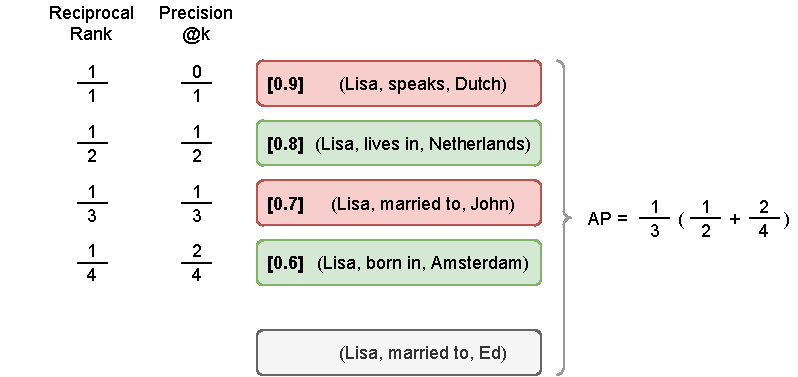
\includegraphics{2_basics/2_metrics/4_map/mrr_map}
    \caption{Calculation of average precision by the example of a list of fact predictions, ranked by confidence. Two of the predictions are relevant (green), two are irrelevant (red) and one relevant fact has been missed out (grey). Average precision would have been optimal if all three relevant facts had been predicted at the top of the list.}
    \label{fig:2_basics/2_metrics/4_map/mrr_map}
\end{figure}

As for MRR, mAP takes values in $(0, 1]$ and is not defined if there are no relevant items for an object. Again, the latter case might be handled by ignoring such objects. When evaluating $n$ objects, each with $AP_i$, where $1 <= i <= n$, \emph{mean average precision (mAP)} is calculated as the mean over all items' average precisions:

\begin{align}
    mAP = \frac{1}{n} \sum_{i=1}^{n} AP_i
    \label{eq:2_basics/2_metrics/4_map/map}
\end{align}


